\section{Appendix Section}
\label{sec:appendix_section}

\subsection{Additional SDFusion Fine-tuning results}

\begin{figure}[h]
  \centering
  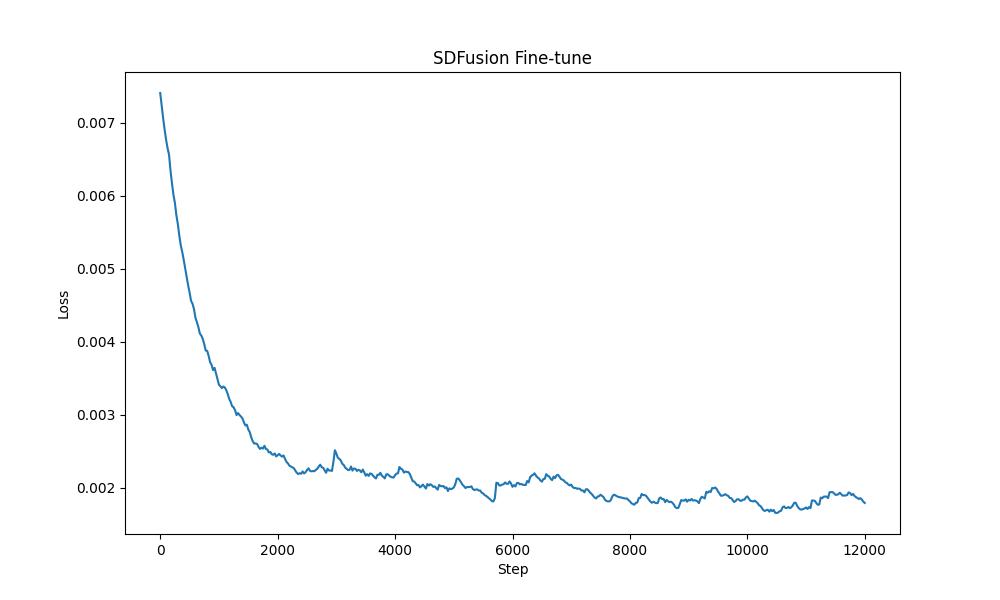
\includegraphics[width=\linewidth]{figs/sdfusion_finetune_loss_plot.png}
  \caption{Loss curve of our SDFusion fine-tune (smoothed).}
  \label{fig:finetune}
\end{figure}

\subsection{Additional Panoptic Model Training Results}

\begin{figure}[h]
  \centering
  \begin{subfigure}[b]{0.45\linewidth}
    \centering
    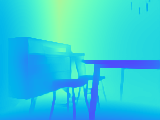
\includegraphics[width=\linewidth]{figs/depth_ours.png}
    \label{subfig:sub1}
   \vspace*{-3mm} % Adjust vertical spacing between the caption and the images
  \caption{Depth map (ours).}
  \end{subfigure}
  \hfill
  \begin{subfigure}[b]{0.45\linewidth}
    \centering
    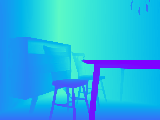
\includegraphics[width=\linewidth]{figs/depth_pan.png}
    \label{subfig:sub2}
   \vspace*{-3mm} % Adjust vertical spacing between the caption and the images
  \caption{Depth map (\citep{dahnert2021panoptic}).}
  \end{subfigure}

  \vspace{0.03\linewidth} % Adjust vertical spacing between rows of figures

  \begin{subfigure}[b]{0.45\linewidth}
    \centering
    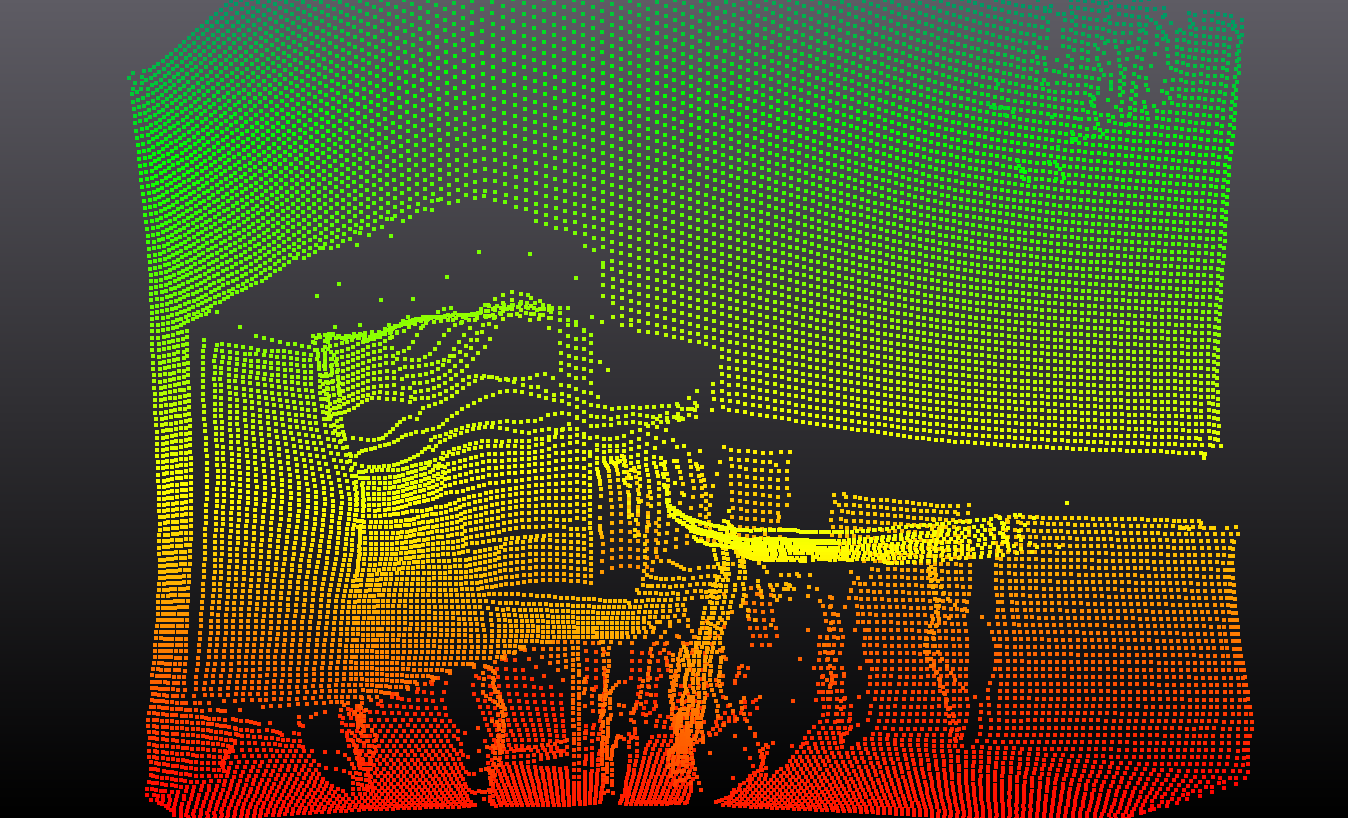
\includegraphics[width=\linewidth]{figs/depthply_ours.png}
    \label{subfig:sub3}
   \vspace*{-3mm} % Adjust vertical spacing between the caption and the images
   \caption{Geometry from depth (ours).}
  \end{subfigure}
  \hfill
  \begin{subfigure}[b]{0.45\linewidth}
    \centering
    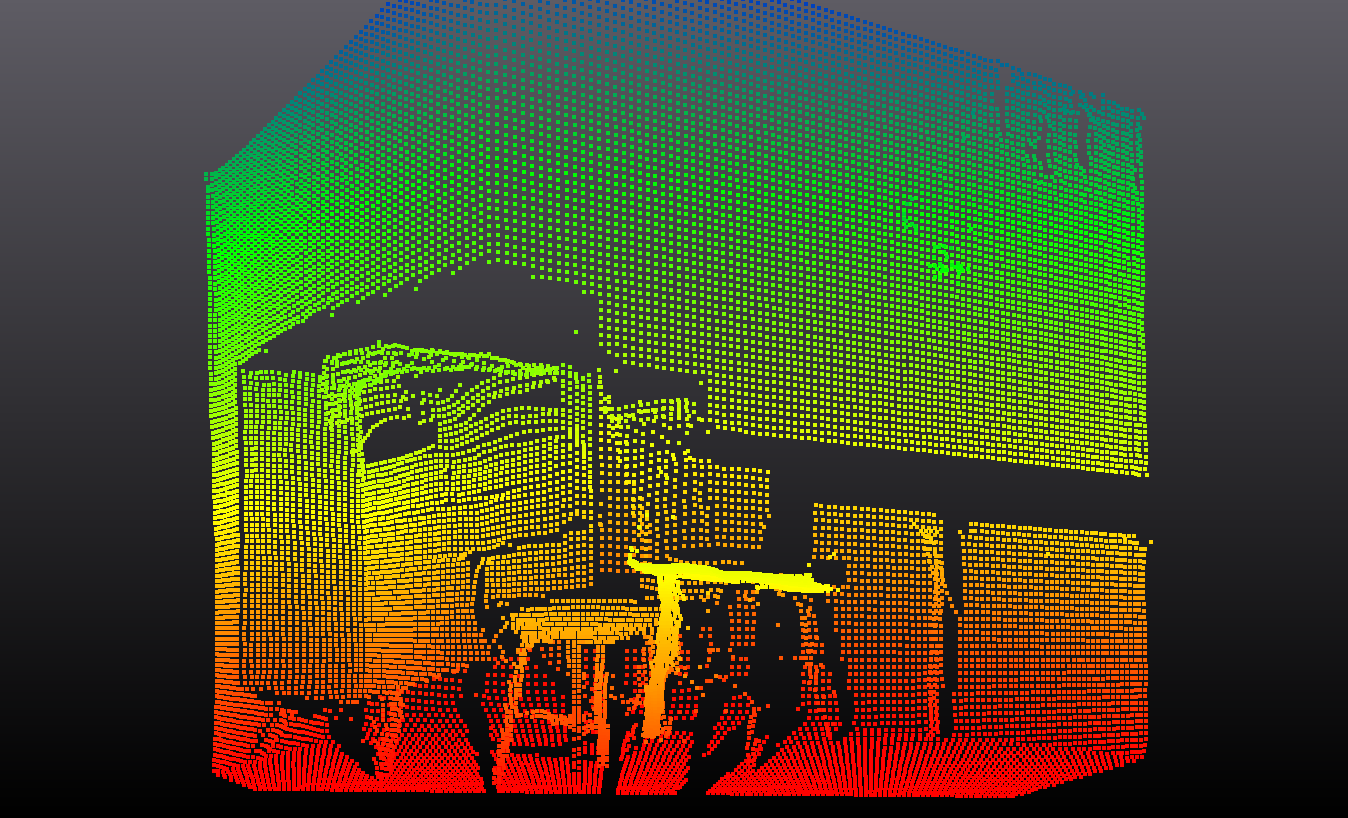
\includegraphics[width=\linewidth]{figs/depthply_pan.png}
    \label{subfig:sub4}
   \vspace*{-3mm} % Adjust vertical spacing between the caption and the images
   \caption{Geometry from depth (\citep{dahnert2021panoptic}).}
  \end{subfigure}

  \caption{2D results from the Panoptic 3D model. Our re-training results (left) vs. results from \citet{dahnert2021panoptic} (right).}
  \label{fig:qual_panoptic}
\end{figure}